\subsection{Fooling Discriminator to Discriminate Original Video from Summary-Based Reconstruction}
\label{section:rel-unsup-discriminative}

\begin{figure}[ht]
    \centering
    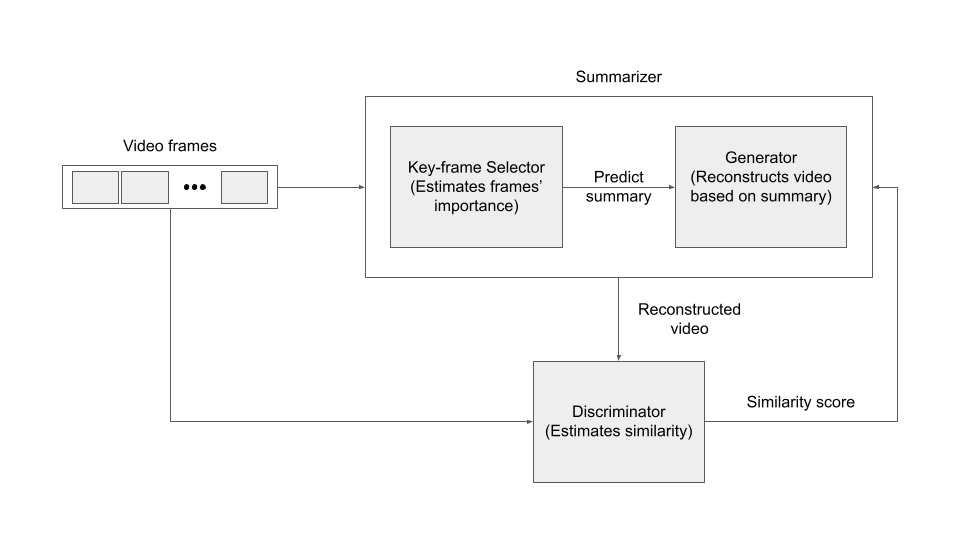
\includegraphics[width=0.73\paperwidth]{content/related/figures/unsup-gan.png}
    \caption{High-level representation of the analysis pipeline of unsupervised
    algorithms that learn summarization by increasing the similarity between the
    summary and the video.}
    \label{figure:rel-unsup-gan}
  \end{figure}

To address the absence of ground-truth data, unsupervised techniques leverage the principle that a representative summary should enable viewers to comprehend the original video content. To achieve this, Generative Adversarial Networks (GANs) are employed to learn the creation of video summaries that facilitate accurate reconstruction of the original video. The training process (see \hyperref[figure:rel-unsup-gan]{Figure \ref{figure:rel-unsup-gan}}) involves a Summarizer, consisting of a Key-frame Selector and a Generator. The Key-frame Selector estimates frame importance and generates a summary, while the Generator reconstructs the video based on the generated summary. By inputting the video frames and predicting frame-level importance scores, the Summarizer reconstructs the original video. The reconstructed video, alongside the original one, is fed into a trainable Discriminator that evaluates their similarity. Similar to supervised GAN-based methods, the training of the entire summarization architecture follows an adversarial approach. In this case, the Summarizer's objective is to deceive the Discriminator by making it challenging to distinguish between the summary-based reconstructed video and the original video. Conversely, the Discriminator aims to improve its discrimination abilities. When the discrimination becomes indistinguishable (i.e., similar classification error for both videos), the Summarizer successfully constructs a highly representative video summary.  

Notably, Mahasseni \etal~\cite{mahasseni2017unsupervised} combined an LSTM-based key-frame selector, a Variational Auto-Encoder (VAE), and a trainable Discriminator, using adversarial learning to minimize the distance between the original video and the summary-based reconstructed version. Building upon this foundation, Apostolidis \etal~\cite{apostolidis2019stepwise} proposed a stepwise, label-based approach for training the adversarial part of the network, leading to enhanced summarization performance. Yuan \etal~\cite{yuan2019cycle} introduced an approach aiming to maximize the mutual information between the summary and the video, utilizing a pair of trainable discriminators and a cycle-consistent adversarial learning objective. Their frame selector, a bidirectional LSTM, constructs a video summary by modeling temporal dependencies among frames. The summary is then evaluated by two GANs—an encoder-decoder GAN for forward reconstruction and a backward GAN for reverse reconstruction. The consistency between these reconstructions quantifies information preservation, guiding the frame selector to identify the most informative frames for the video summary. In a subsequent work, Apostolidis \etal~cite{apostolidis2020ac} integrated an Actor-Critic model into a GAN, formulating the selection of important video fragments as a sequence generation task. The Actor and Critic engage in a game that incrementally selects video key fragments, with rewards from the Discriminator influencing their choices. This training workflow enables the Actor and Critic to learn a value function (Critic) and a policy for key-fragment selection (Actor). Other approaches extended the core VAE-GAN architecture by incorporating tailored attention mechanisms. For instance, Jung \etal~\cite{jung2019discriminative} proposed a VAE-GAN architecture extended with a chunk and stride network (CSNet) and a tailored difference attention mechanism, capturing frame dependencies at various temporal granularities during keyframe selection. In a subsequent work, Jung \etal~\cite{jung2020global} introduced a self-attention mechanism combined with relative position modeling, decomposing the frame sequence into non-overlapping groups to capture both local and global interdependencies. Apostolidis \etal~\cite{apostolidis2020unsupervised} presented a variation of their prior work \cite{apostolidis2019stepwise}, replacing the VAE with a deterministic Attention Auto-Encoder to improve attention-driven reconstruction and key-fragment selection. He \etal~\cite{he2019unsupervised} proposed a self-attention-based conditional GAN, utilizing a conditional feature selector and a multi-head self-attention mechanism to focus on important temporal regions and model long-range dependencies in the video sequence. Finally, Rochan \etal~\cite{rochan2019video} developed an approach for video summarization from unpaired data, employing an adversarial process with GANs and a Fully-Convolutional Sequence Network (FCSN) encoder-decoder. The model aimed to learn a mapping function from raw video to a human-like summary, aligning the summary distribution with human-created summaries while ensuring content diversity through an applied constraint on the learned mapping function.

These techniques aim to generate representative video summaries by fooling the Discriminator, making it difficult to distinguish between the summary-based reconstruction and the original video. By achieving similar classification errors for both, it indicates that the Summarizer has successfully created a summary that captures the overall video content.